\chapter{A new proprioceptive and vision dataset}
\label{chp:dataset}

This short chapter presents a dataset that we recently produced with Gepetto team's quadruped robot Solo-12. This dataset was acquired in our experimental space 
in LAAS-CNRS (see \figRef{fig:solo_dataset_scene}) and includes several walking trajectories using the controller \cite{leziart2021implementation}. We remote-controlled the robot in a scene augmented 
with \apriltags\ and elements from the T-less dataset, recording proprioceptive and exteroceptive measurements. 

\begin{figure}[h]
    \centering
    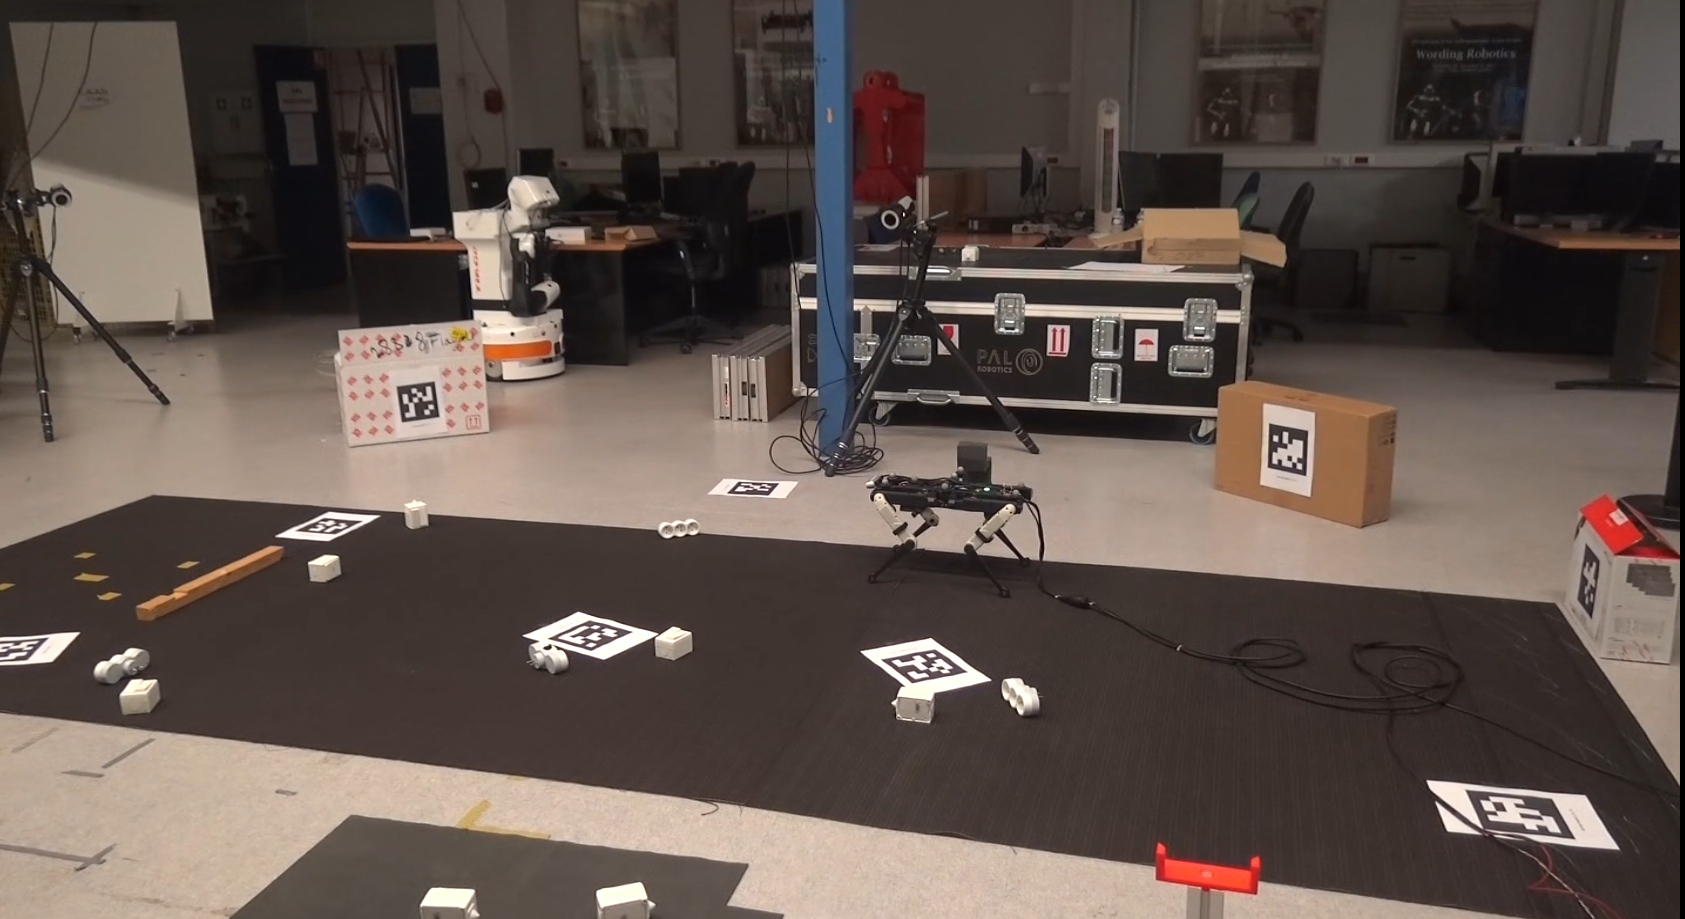
\includegraphics[width=0.95\textwidth]{figures/solo_dataset_scene.png}
    \caption{Solo quadruped in the experimental room.}
    \label{fig:solo_dataset_scene}
\end{figure}

The recorded sensor measurements include joint encoders, joint currents, the IMU from Solo onboard sensing as well as RGB camera and IMU from a RealSense D435i.
Controller logs (such as the planned feet contacts timings) are also recorded. The RealSense was fixed at the front of the robot, slightly down-facing (30 degrees).
A summary of available data is reported in \tabRef{tab:dataset_solo}. Calibration data using a fiducial marker grid were recored before the experiments to 
obtain the image distortion, camera-IMU relative transformation, and potential time-shift of the RealSense system. A sample image of one of the trajectories
is shown in \figRef{fig:solo_dataset_image}.
External video recordings of each experiment were taken.

\begin{table}[h]
    \centering
    \caption{Summary of available data sources from Solo-12 onboard sensing and RealSense D435i}
    \begin{tabular}{|llll|}
        \hline
        \thead[l]{Type} & \thead[l]{Source} & \thead[l]{Details} & \thead[l]{Frequency}  \\
        \hline
        Joint currents & Solo-12 &  & 1 kHz  \\
        \hline
        IMU            & Solo-12 & \makecell[l]{3DM-CX5-25 \\ LORD Microstrain} & 1 kHz  \\
        \hline
        RGB images & Solo-12 & \makecell[l]{1920 × 1080 \\ rolling shutter} & 30 Hz  \\
        \hline
        IMU            & RealSense & Bosch BMI055 & 200 Hz  \\
        \hline
        Ground truth & Qualysis Motion Capture &  & 200 Hz \\
        \hline
    \end{tabular}
    \label{tab:dataset_solo}
\end{table}


All data from Solo's onboard sensing is hardware synchronized. Similarly, the RealSense IMU and RGB images streams are synchronized. However, 
we do not have the possibility to hardware synchronize the RealSense with Solo yet. Instead, we plan to rely on the correlation between Solo's IMU and the RealSense IMU
to synchronize the streams of data in a post-processing step. To this end, we proceeded to a synchronization procedure at the beginning of each trajectory by
tapping on the robot a few times. This precise signal should be enough to align both IMU time series and, thus, the rest of the sensor streams.


Recorded trajectories (2 minutes each) include motions of increasing difficulty, with forward-backward walking in a straight line, a square path around the scene, and
loopy trajectories. With this dataset, we plan to implement an estimator fusing inertial, kinematics, and object-level transformation based on our previous work.
This will serve to benchmark an integration work destined to obtain an estimator for both balance control states (orientation, velocity) and 
global localization through object-level SLAM. The loopy trajectories in particular will serve to display the behavior of the estimator when closing longer loops.


\begin{figure}[h]
    \centering
    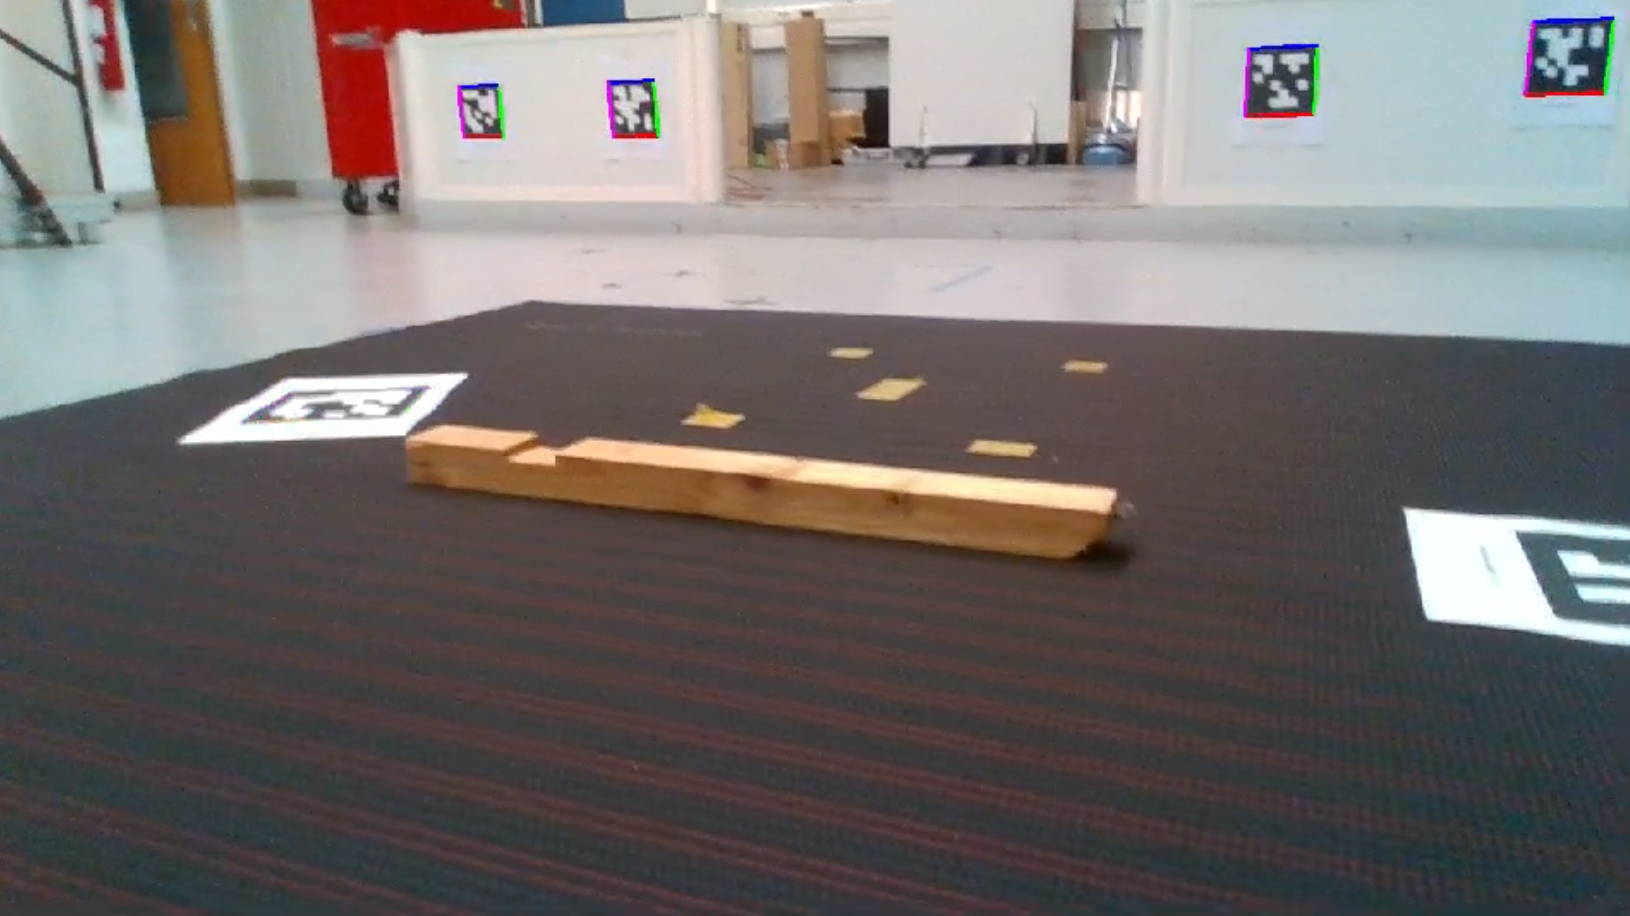
\includegraphics[width=0.7\textwidth]{figures/solo_dataset_image.png}
    \caption{Example of an image captured with the RealSense attached to Solo while walking (with \apriltag\ detections).}
    \label{fig:solo_dataset_image}
\end{figure}